\documentclass{standalone}
\usepackage{tikz}
\usetikzlibrary{shapes.geometric}
\usetikzlibrary{arrows.meta}
\usetikzlibrary{calc}
\usetikzlibrary{backgrounds}
% Define muted colors.
\definecolor{TolMutedBlue}{HTML}{332288}
\definecolor{TolMutedCyan}{HTML}{88CCEE}
\definecolor{TolMutedTeal}{HTML}{44AA99}
\definecolor{TolMutedGreen}{HTML}{117733}
\definecolor{TolMutedOlive}{HTML}{999933}
\definecolor{TolMutedSand}{HTML}{DDCC77}
\definecolor{TolMutedRose}{HTML}{CC6677}
\definecolor{TolMutedWine}{HTML}{882255}
\definecolor{TolMutedPurple}{HTML}{AA4499}
\begin{document}
    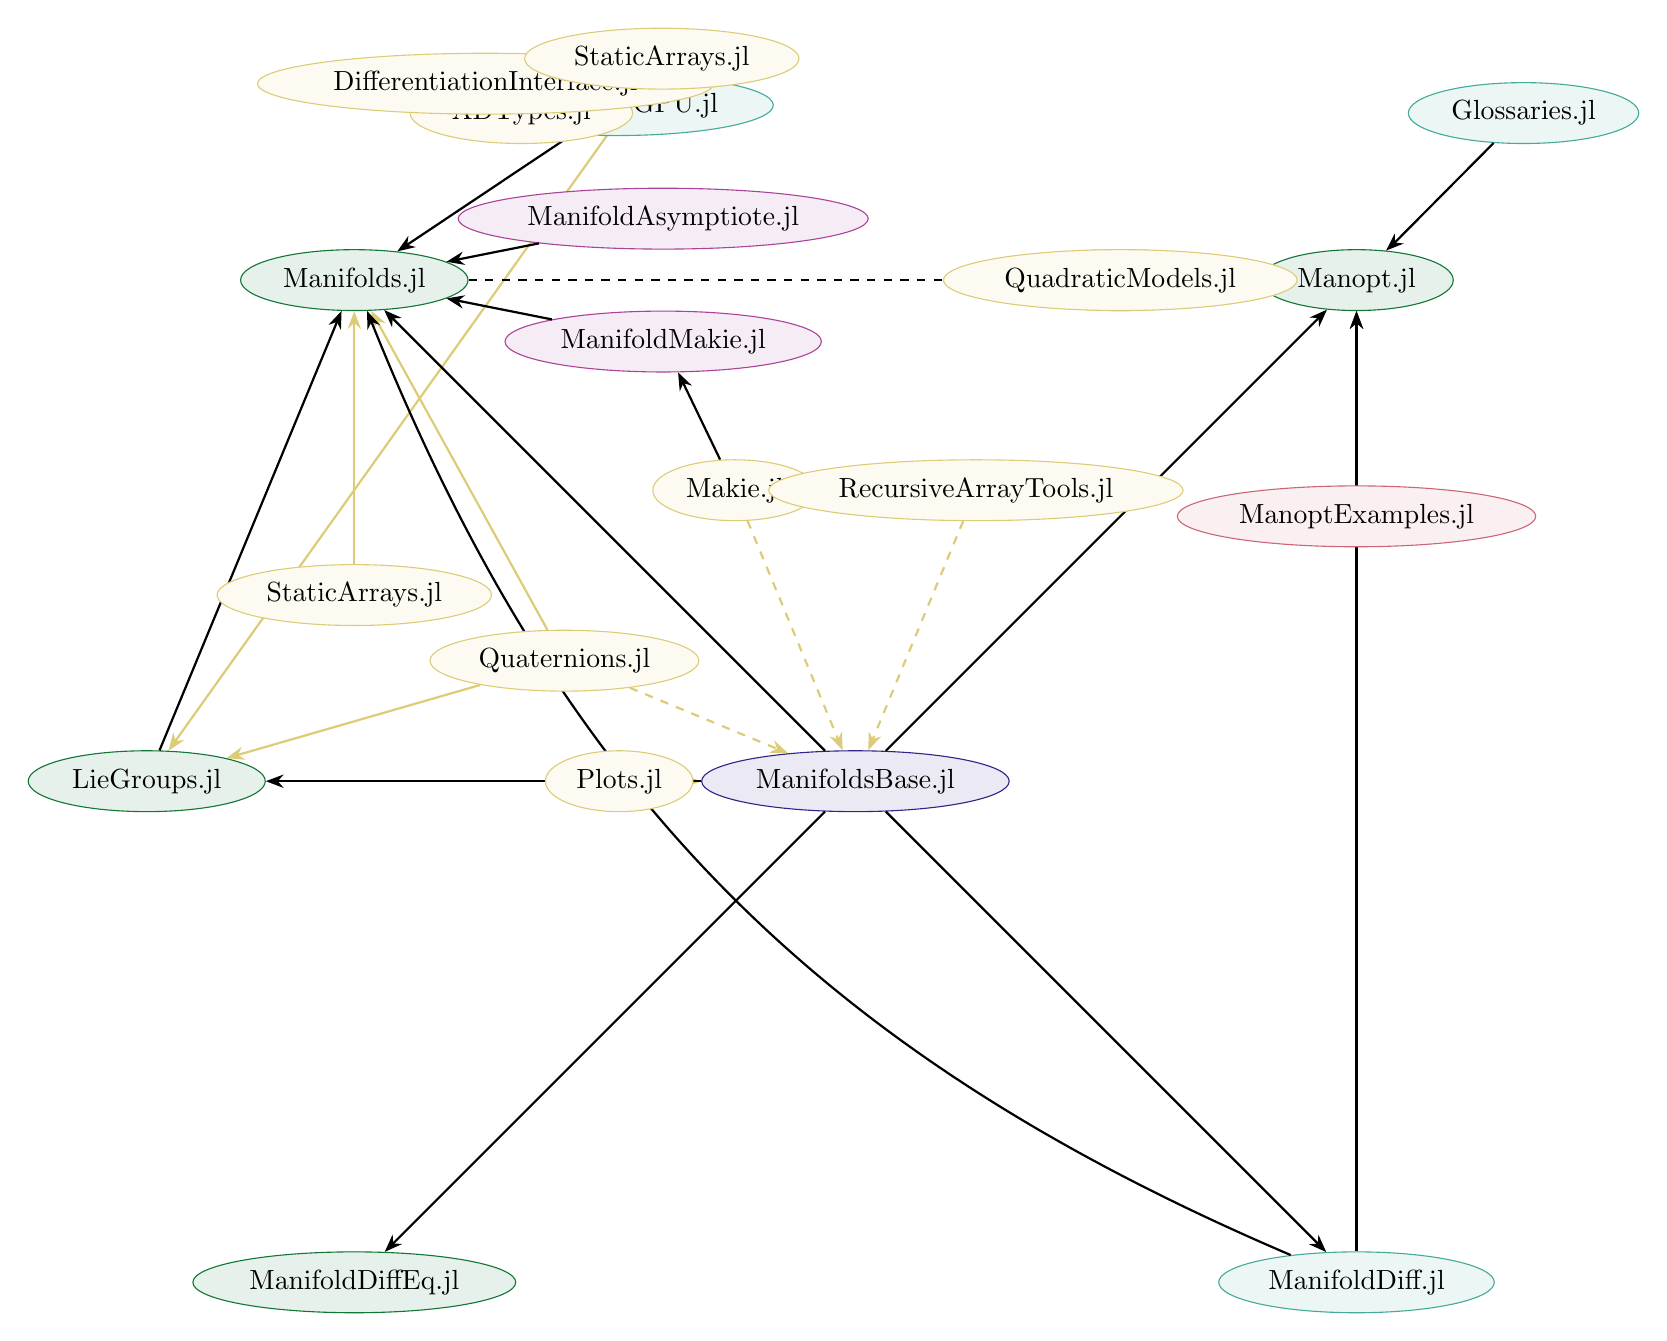
\begin{tikzpicture}
        % Styles of nodes
        \tikzset{Base/.style={draw=TolMutedBlue, fill=TolMutedBlue!10, ellipse}}
        \tikzset{Library/.style={draw=TolMutedGreen, fill=TolMutedGreen!10, ellipse}}
        \tikzset{Func/.style={draw=TolMutedTeal, fill=TolMutedTeal!10, ellipse}}
        \tikzset{Vis/.style={draw=TolMutedPurple, fill=TolMutedPurple!10, ellipse}}
        \tikzset{Examples/.style={draw=TolMutedRose, fill=TolMutedRose!10, ellipse}}
        \tikzset{External/.style={draw=TolMutedSand, fill=TolMutedSand!10, ellipse}}
        % Styles of lines
        % format: a -- B ABExt loading B extends A
        \tikzset{extends/.style={dashed, -{Stealth[length=2.25mm]}, thick}}
        % V2: to external packages
        \tikzset{extends2/.style={dashed, -{Stealth[length=2.25mm]}, thick, TolMutedSand}}
        % format A -- B A is a dependency of B, we draw B-->A
        \tikzset{depends/.style={solid, {Stealth[length=2.25mm]}-,thick}}
        % V2: to external packages
        \tikzset{depends2/.style={solid, {Stealth[length=2.25mm]}-,thick, TolMutedSand}}
        \node[Base] (MB) at (0,0) {ManifoldsBase.jl};
        %
        % Ring I: Core packages
        \node[Library] (M) at ($(MB) + (135:9cm)$) {Manifolds.jl};
        \node[Library] (MO) at ($(MB) + (45:9cm)$) {Manopt.jl};
        \node[Library] (LG) at ($(MB) + (180:9cm)$) {LieGroups.jl};
        \node[Library] (MDE) at ($(MB) + (225:9cm)$) {ManifoldDiffEq.jl};
        \node[Func] (MD) at ($(MB) + (315:9cm)$) {ManifoldDiff.jl};
        \draw[depends] (M) -- (MB);
        \draw[depends] (MO) -- (MB);
        \draw[depends] (MO) -- (MD);
        \draw[depends] (LG) -- (MB);
        \draw[depends] (M) -- (LG);
        \draw[depends] (MDE) -- (MB);
        \draw[depends] (MD) -- (MB);
        \draw[depends] (M) to[bend right=22.5] (MD);
        \draw[extends] (M) -- (MO);
        % Ring II
        %
        % Same direction as Manopt continued
        \node[Examples] (MOE) at ($(MO) + (270:3cm)$) {ManoptExamples.jl};
        \draw[depends] (MO) -- (MOE);
        %
        % Sidequest: Glossaries
        \node[Func] (G) at ($(MO) + (45:3)$) {Glossaries.jl};
        \draw[depends] (MO) -- (G);
        % \node[Base] (AI) at ($(MB) + (270:6.5cm)$) {AlgorithmInterface.jl};

        %
        % Sidequest Viz
        \node[Vis] (MA) at ($(M) + (11.25:4cm)$) {ManifoldAsymptiote.jl};
        \draw[depends] (M) -- (MA);
        \node[Vis] (MM) at ($(M) + (348.75:4cm)$) {ManifoldMakie.jl};
        \draw[depends] (M) -- (MM);
        \node[Func] (MG) at ($(M) + (33.75:4cm)$) {ManifoldsGPU.jl};
        \draw[depends] (M) -- (MG);
        \node[External] (Makie) at ($(MB) + (112.5:4)$) {Makie.jl};
        \begin{pgfonlayer}{background}
             \draw[depends] (MM) -- (Makie);
        \end{pgfonlayer}
        %
        %
        % dependencies of ManifoldsBase.jl that are not the base language
        % excluded: LinearAlgebra, Markdown, Preferences, Printf, Random
        % weak dependencies
        \node[External] (Plots) at ($(MB) + (180:3)$) {Plots.jl};
        \node[External] (Quat) at ($(MB) + (157.5:4)$) {Quaternions.jl};
        \node[External] (RAT) at ($(MB) + (67.5:4)$) {RecursiveArrayTools.jl};
        % Excluded: Statistics
        \begin{pgfonlayer}{background}
             \draw[extends2] (Makie) -- (MB);
             \draw[extends2] (Plots) -- (MB);
             \draw[extends2] (Quat) -- (MB);
             \draw[extends2] (RAT) -- (MB);
        \end{pgfonlayer}%
        %
        %
        % Dependencies for Manifolds.jl
        % already existing: Quaternions, ManifoldDiff, ManifoldsBase
        \node[External] (AD) at ($(M) + (45:3)$) {ADTypes.jl};
        \node[External] (DI) at ($(M) + (56.25:3)$) {DifferentiationInterface.jl};
        %\node[External] (Gr) at ($(M) + (101.25:3)$)  {Graphs.jl};
        %\node[External] (Kr) at ($(M) + (112.5:3)$)  {Kronecker.jl};
        %\node[External] (MatEq) at ($(M) + (124.75:3)$)  {MatrixEquations.jl};
        %\node[External] (SF) at ($(M) + (180:3)$)  {SpecialFunctions.jl};
        %\node[External] (SWG) at ($(M) + (180:3)$)  {SimpleWeightedGraphs.jl};
        \node[External] (SA) at ($(M) + (270:4)$) {StaticArrays.jl};
        %\node[External] (SB) at ($(M) + (180:3)$)  {StatsBase.jl};
        %\node[External] (Tullio) at ($(MO) + (180:3)$)  {Tullio.jl};
        % excluded: LinearAlgebra, Markdown, Preferences, Printf, Random, Statistics
        \begin{pgfonlayer}{background}
             \draw[depends2] (M) -- (Quat);
             \draw[depends2] (M) -- (SA);
        \end{pgfonlayer}
        %
        %
        % Dependencies for Manopt.jl
        % already existing: Glossaires, ManifoldDiff, ManifoldsBase
        \node[External] (SA) at (105:9.5) {StaticArrays.jl};
        % excluded: DataStructures, Dates, Markdown, Preferences, Printf, Random, Statistics
        % weak dependencies
        % already existing: Manifolds, RAT
        \node[External] (LRU) at ($(MO) + (180:3)$) {LRUCaches.jl};
        \node[External] (LS) at ($(MO) + (180:3)$) {Linesearches.jl};
        \node[External] (RipQP) at ($(MO) + (180:3)$) {RipQP.jl};
        \node[External] (QM) at ($(MO) + (180:3)$) {QuadraticModels.jl};
        %
        %
        % dependencies of LieGroups.jl that are not the base language
        % excluded: LinearAlgebra, Random
        % already existing: Manifolds, ManifoldsBase, Quaternions, StaticArrays
        % weak dependencies
        % Excluded: Statistics
        \begin{pgfonlayer}{background}
             \draw[depends2] (LG) -- (Quat);
             \draw[depends2] (LG) -- (SA);
        \end{pgfonlayer}


        % already excluded: JuMP (since soon removed)
        % Extensions and outer packages on a large circle
        % \node[External] (Asymptote) at (120:9.5) {Asymptote.jl};
        % \node[External] (Test) at (150:9.5) {Test.jl};
        % \node[External] (RAT) at (195:9.5) {RecursiveArrayTools.jl};
        % \node[External] (SLMB) at (270:9.5) {SciMLBase.jl};
        % \node[External] (ODE) at (285:9.5) {OrdinaryDiffEq.jl};
        % \node[External] (NLS) at (300:9.5) {NLSolve.jl};
        % \node[External] (MIRK) at (315:9.5) {BoundaryValueDiffEqMIRK.jl};
        % \node[External] (RipQP) at (330:9.5) {RipQP.jl};
        % \node[External] (QM) at (345:9.5) {QuadraticModels.jl};
        % \node[External, text width=2.8cm, align=center] (Diffs) at (222.5:12.5) {FiniteDiff.jl\\FiniteDifferences.jl\\ForwardDiff.jl\\ReverseDiff.jl\\Zygote.jl};
        % \draw[depends2] (MA) -- (Asymptote);
        % \draw[depends2] (MM) -- (Makie);
        \begin{pgfonlayer}{background}
        %     \draw[depends] (MD) to [bend right=50] (MOE);
        %     %
        %     \draw[extends2] (Test) -- (M);
        %     \draw[extends2] (Test) -- (LG);
        %     \draw[extends2] (Plots) -- (MB);
        %     \draw[extends2] (Plots) -- (M);
        %     \draw[extends2] (Makie) -- (MB);
        %     \draw[extends2] (Quat) -- (MB);
        %     \draw[extends2] (RAT) -- (M);
        %     \draw[extends2] (RAT) -- (MB);
        %     \draw[extends2] (RAT) -- (LG);
        %     \draw[depends2] (M) to (Quat);
        %     \draw[depends2] (M) -- (Gr);
        %     \draw[depends2] (M) -- (Kr);
        %     \draw[depends2] (M) -- (SWG);
        %     \draw[depends2] (M) -- (SF);
        %     \draw[depends2] (M) -- (Tullio);
        %     \draw[depends2] (M) -- (SB);
        %     \draw[depends2] (M) to [bend left=22.5] (MatEq);
        %     \draw[depends2] (M) to [bend left=22.5] (SA);
        %     \draw[depends2] (LG) to [bend left=22.5] (SA);
        %     % Manopt extensions
        %     \draw[extends2] (RAT) -- (MO);
        %     \draw[extends2] (RipQP) -- (MO);
        %     \draw[extends2] (QM) -- (MO);
        %     \draw[extends2] (LRU) -- (MO);
        %     \draw[extends2] (LS) -- (MO);
        %     % ManifoldDiff dependencies
        %     \draw[depends2] (MD) -- (AD);
        %     \draw[depends2] (MD) -- (DI);
        %     \draw[depends2] (MD) -- (AD);
        %     \draw[depends2] (MD) -- (AD);
        %     \draw[extends2] (Diffs) to [bend left = 12.75] (MD);
        %     % ManifoldDiffEq dependencies
        %     \draw[depends2] (MDE) -- (M);
        %     \draw[depends2] (MDE) -- (ODE);
        %     \draw[depends2] (MDE) to [bend left=22.5] (RAT);
        %     \draw[depends2] (MDE) -- (SLMB);
        \end{pgfonlayer}
    \end{tikzpicture}
\end{document}